\clearpage
\section{Results}

It is challenging to get the network to learn stable and well. Here I present the learning process for various sizes of the replay buffer and look at the effect of infrequent weight updating. I take a look at what these changes mean for learning stability. The parameters in \autoref{tab:shared_params} are shared between all results. The results are presented in figures containing a pair of runs. Each run has the value of epsilon, the score for each iteration and the moving average\footnote{we use a window of 50 training iterations} of the score. The moving average will help recognize medium term unstable learning.

\begin{table}[ht]
  \centering
  \fontfamily{ppl}\selectfont
  \begin{tabular}{ll}
    \toprule
    Paramater & Value \\
    \midrule
    discount factor $\gamma$ & $0.95$ \\
    replay sample size & $32$ \\
    maximum steps & $200$ \\
    training iterations & $1000$ \\
    learning rate & $0.001$ \\
    epsilon start & $5$ \\
    epsilon decay & $5^{-5}$ \\
    \bottomrule
  \end{tabular}
  \caption{The parameters and their values shared between all mountain car results.}
  \label{tab:shared_params}
\end{table}

The default size of the replay buffer is $20000$ time steps or events. I start by looking at the learning behavior of the agent with this size of buffer. Because reinforced learning can be unrepeatable, especially when combined with the unrepeatable of neural networks I train the agent 4 times. 

\begin{figure}
    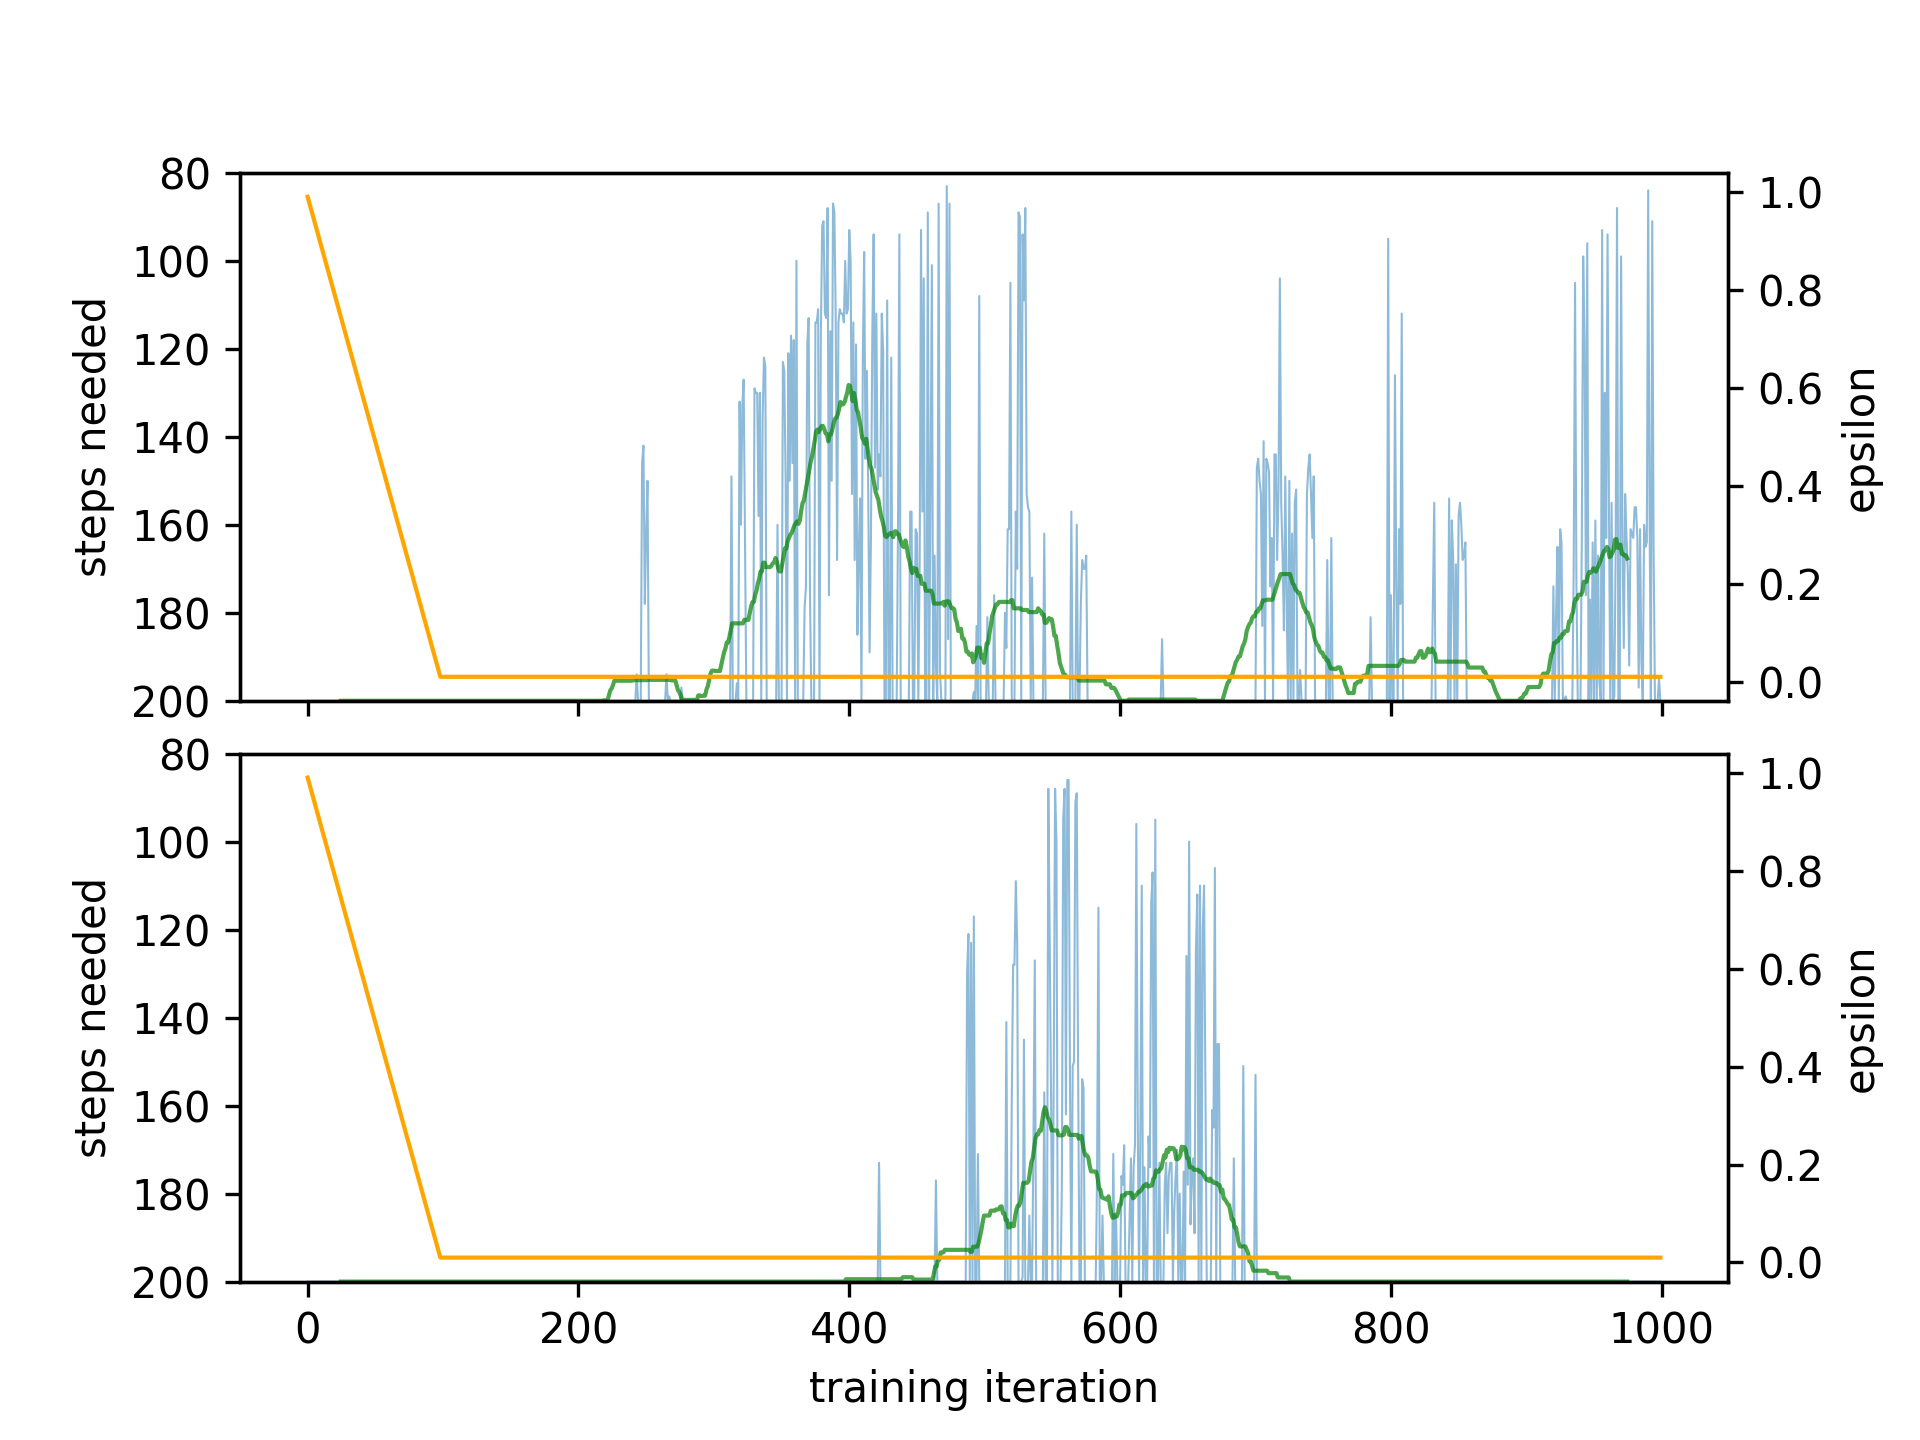
\includegraphics{mcar_20000_a}
    \caption{Two separate runs of training the mountain car agent with a replay buffer which remembers the last $20000$ time steps. On the y-axis the number of steps needed to finish, 200 means the algorithm failed to reach the goal in time. On the x-axis the iteration number. The orange line is epsilon, the blue line follows the scores of the training iteration and the green line is the moving average of the score. Note how both attempts do not lead to convergence within 1000 steps}
    \label{fig:mcar_20k_a}
\end{figure}

\begin{figure}
    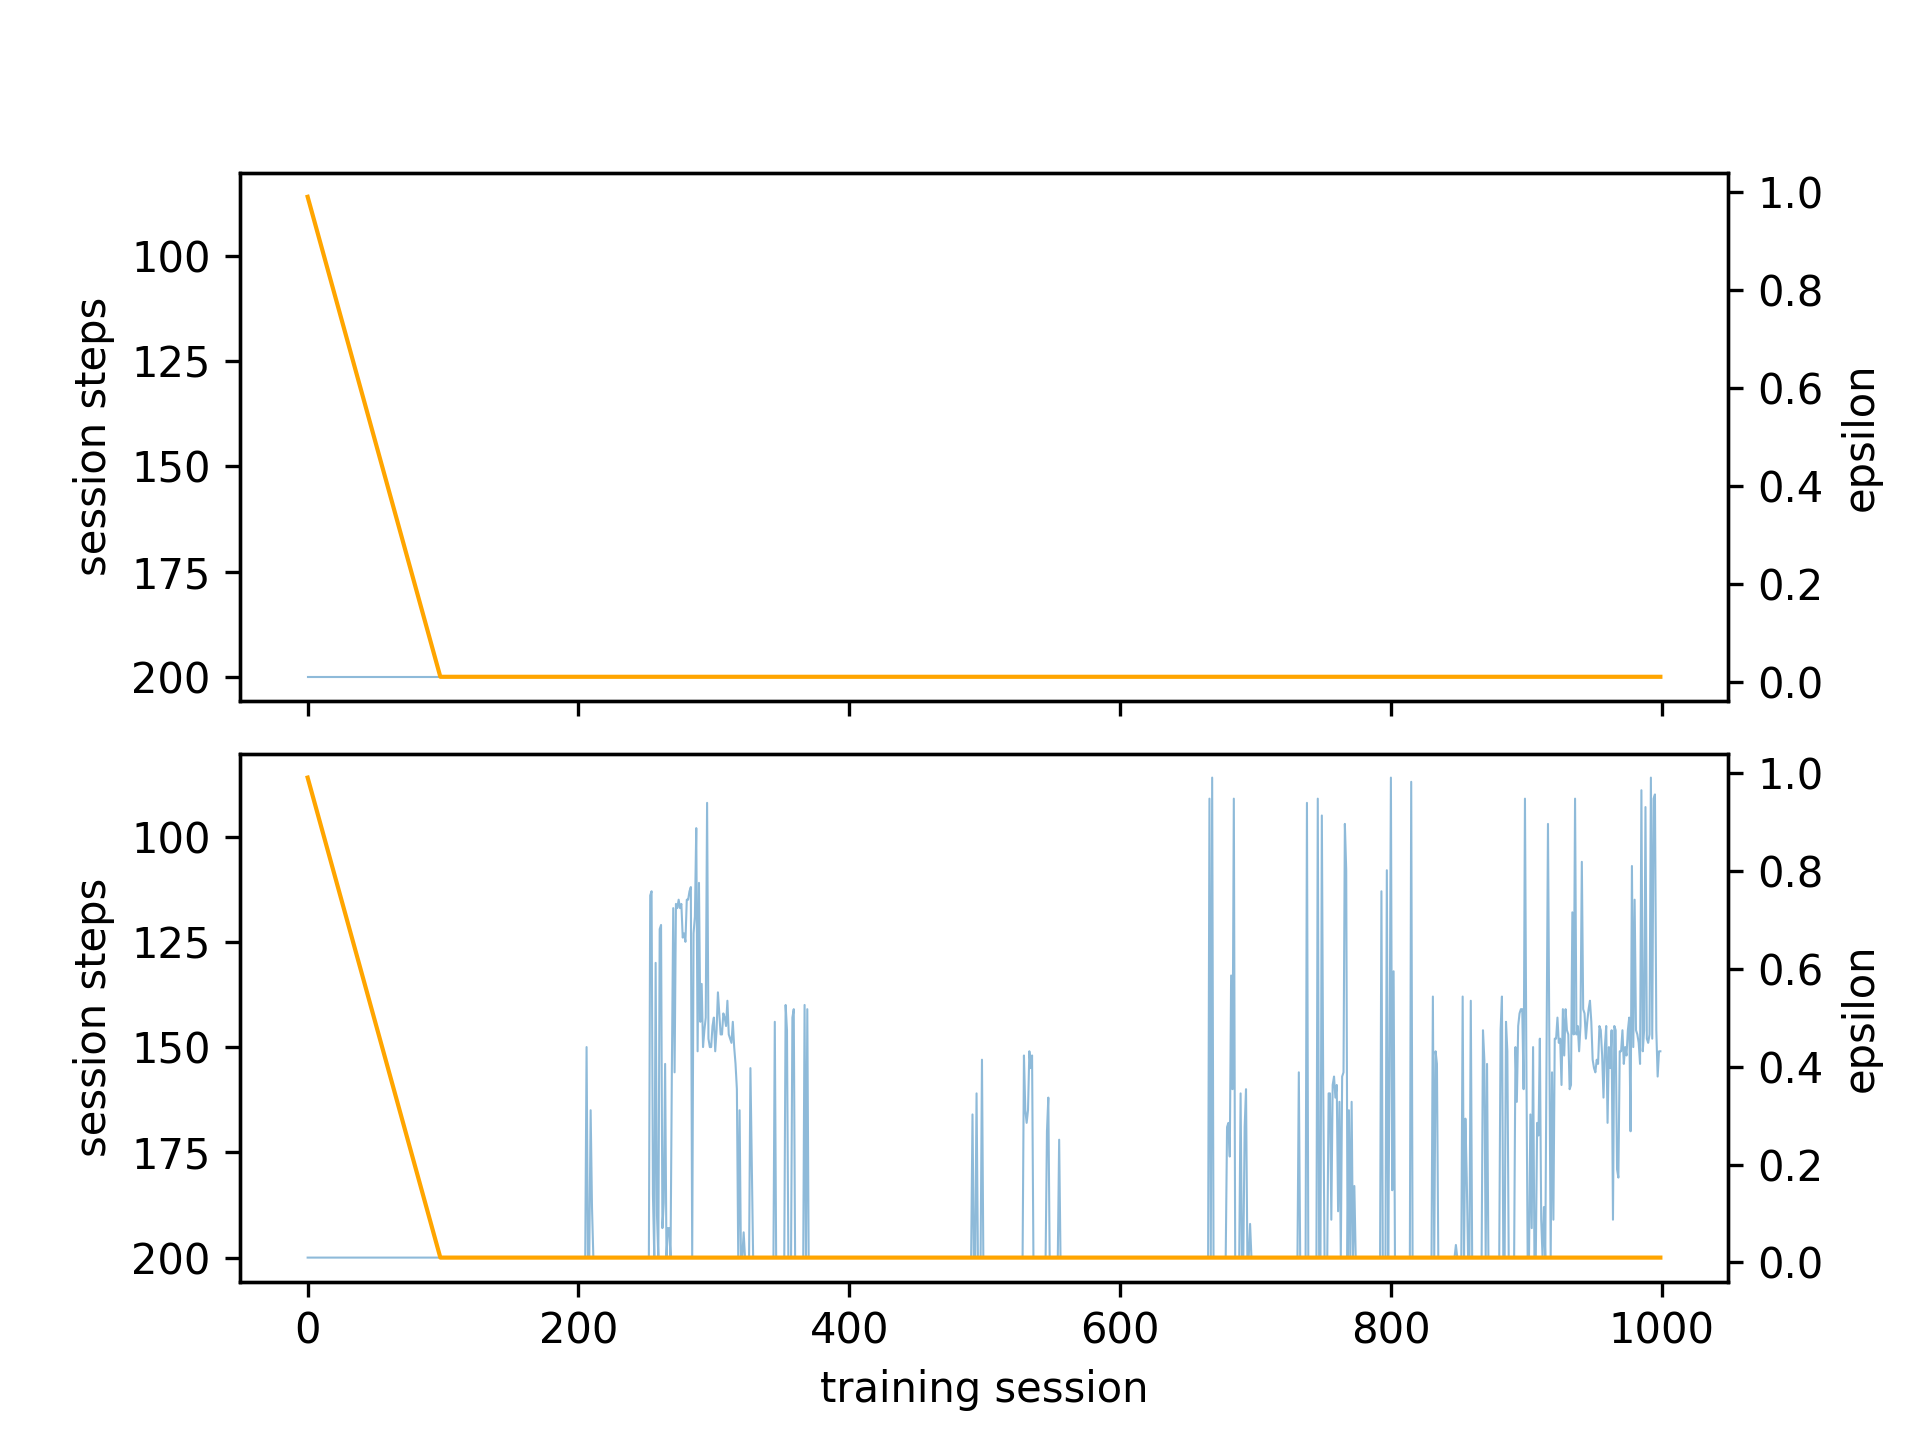
\includegraphics{mcar_20000_b}
    \caption{One run of training the mountain car agent with a replay buffer which remembers the last $20000$ time steps. On the y-axis the number of steps needed to finish, 200 means the algorithm failed to reach the goal in time. On the x-axis the iteration number. The orange line is epsilon, the blue line follows the scores of the training iteration and the green line is the moving average of the score. Note that agent seems to converge at around iteration 900.}
    \label{fig:mcar_20k_b}
\end{figure}

One of the times the agents did not solve the problem once using the maximum of $200$ steps each iteration, the three successful results are in \autoref{fig:mcar_20k_a} and \autoref{fig:mcar_20k_b}. The agent is unstable it can start producing good results before failing at the task again 200 training iterations later as seen in the bottom plot of \autoref{fig:mcar_20k_a}

Now I look at the learning stability of the agent if I decrease the buffer size, I expect the stability to decrease as the famous deadly triad becomes a larger problem and the agent starts biting in its own tail more. In \autoref{fig:mcar_10k_a} and \autoref{fig:mcar_10k_b} we see the learning behavior of the agents with a replay buffer of $10 000$ time steps.

\begin{figure}
    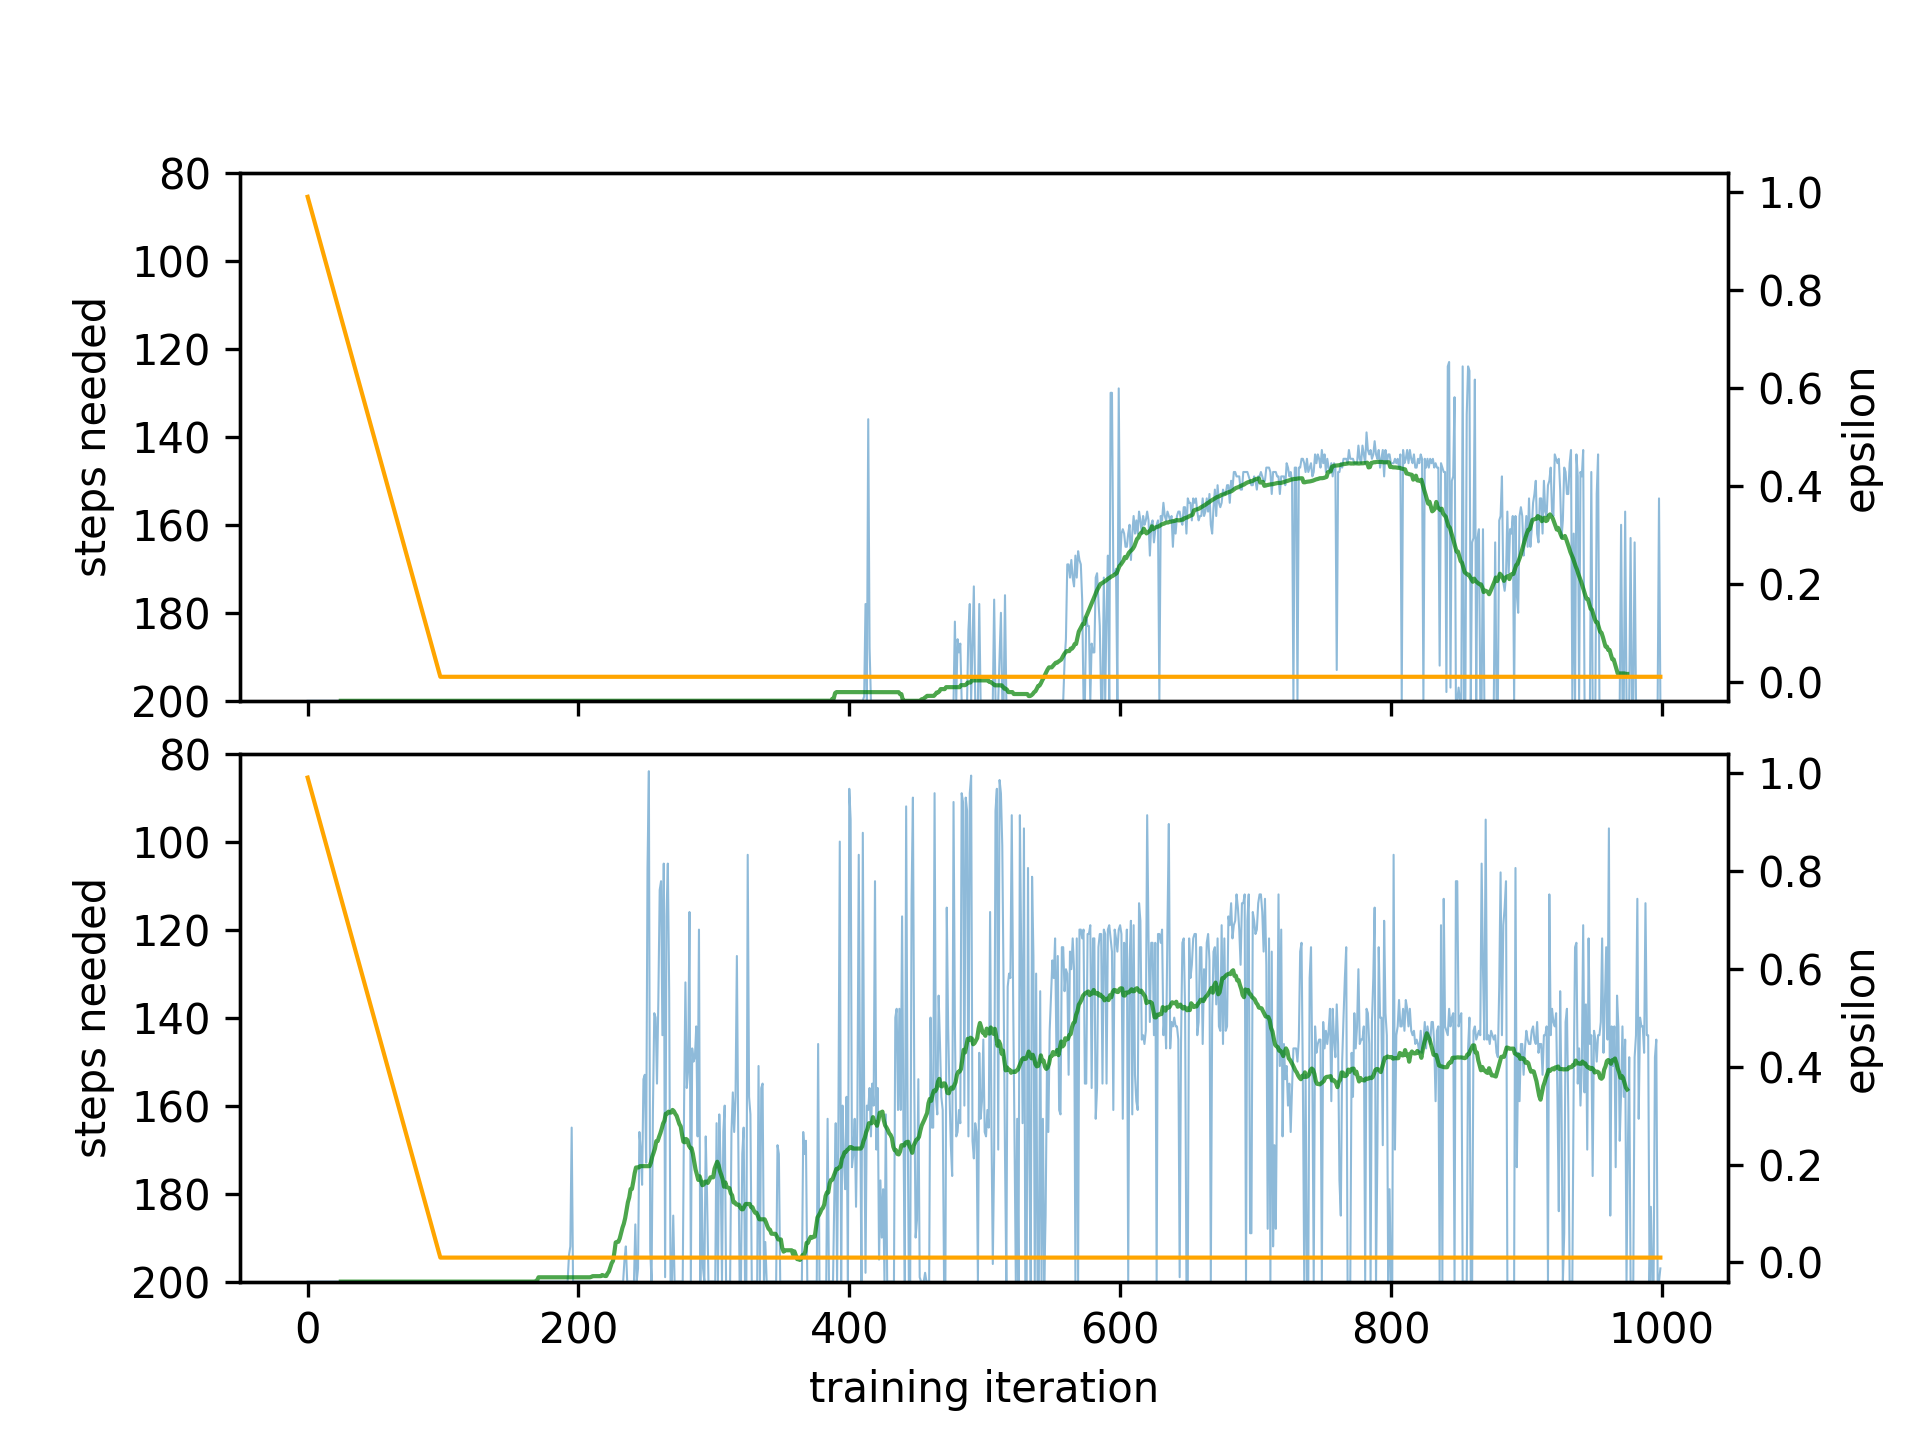
\includegraphics{mcar_10000}
    \caption{Two separate runs of training the mountain car agent with a replay buffer which remembers the last $10000$ time steps. On the y-axis the number of steps needed to finish, 200 means the algorithm failed to reach the goal in time. On the x-axis the iteration number. The orange line is epsilon, the blue line follows the scores of the training iteration and the green line is the moving average of the score. The first run in the top part of this plot shows stability improving as the training iterations continue. Note in the second run (bottom part of figure) the seemingly stable behavior improving slowly   before collapsing. The overall performance is worse then that of any of the other successful runs.}
    \label{fig:mcar_10k_a}
\end{figure}

In the upper part of figure \autoref{fig:mcar_10k_a} we see the agent grow stably become better between episode 600 and 800 before collapsing. In the lower part of that figure the agent is behaving more stable as the training iterations go on. In half of the runs the agent failed to complete the task once within the available time ($200$ time steps).

Doubling the replay buffer size from the default to $40 000$ time steps gives rise to the results in \autoref{fig:mcar_40k_a} and \autoref{fig:mcar_40k_b}. By increasing the replay buffer size I expect more stable behavior. 

\begin{figure}
    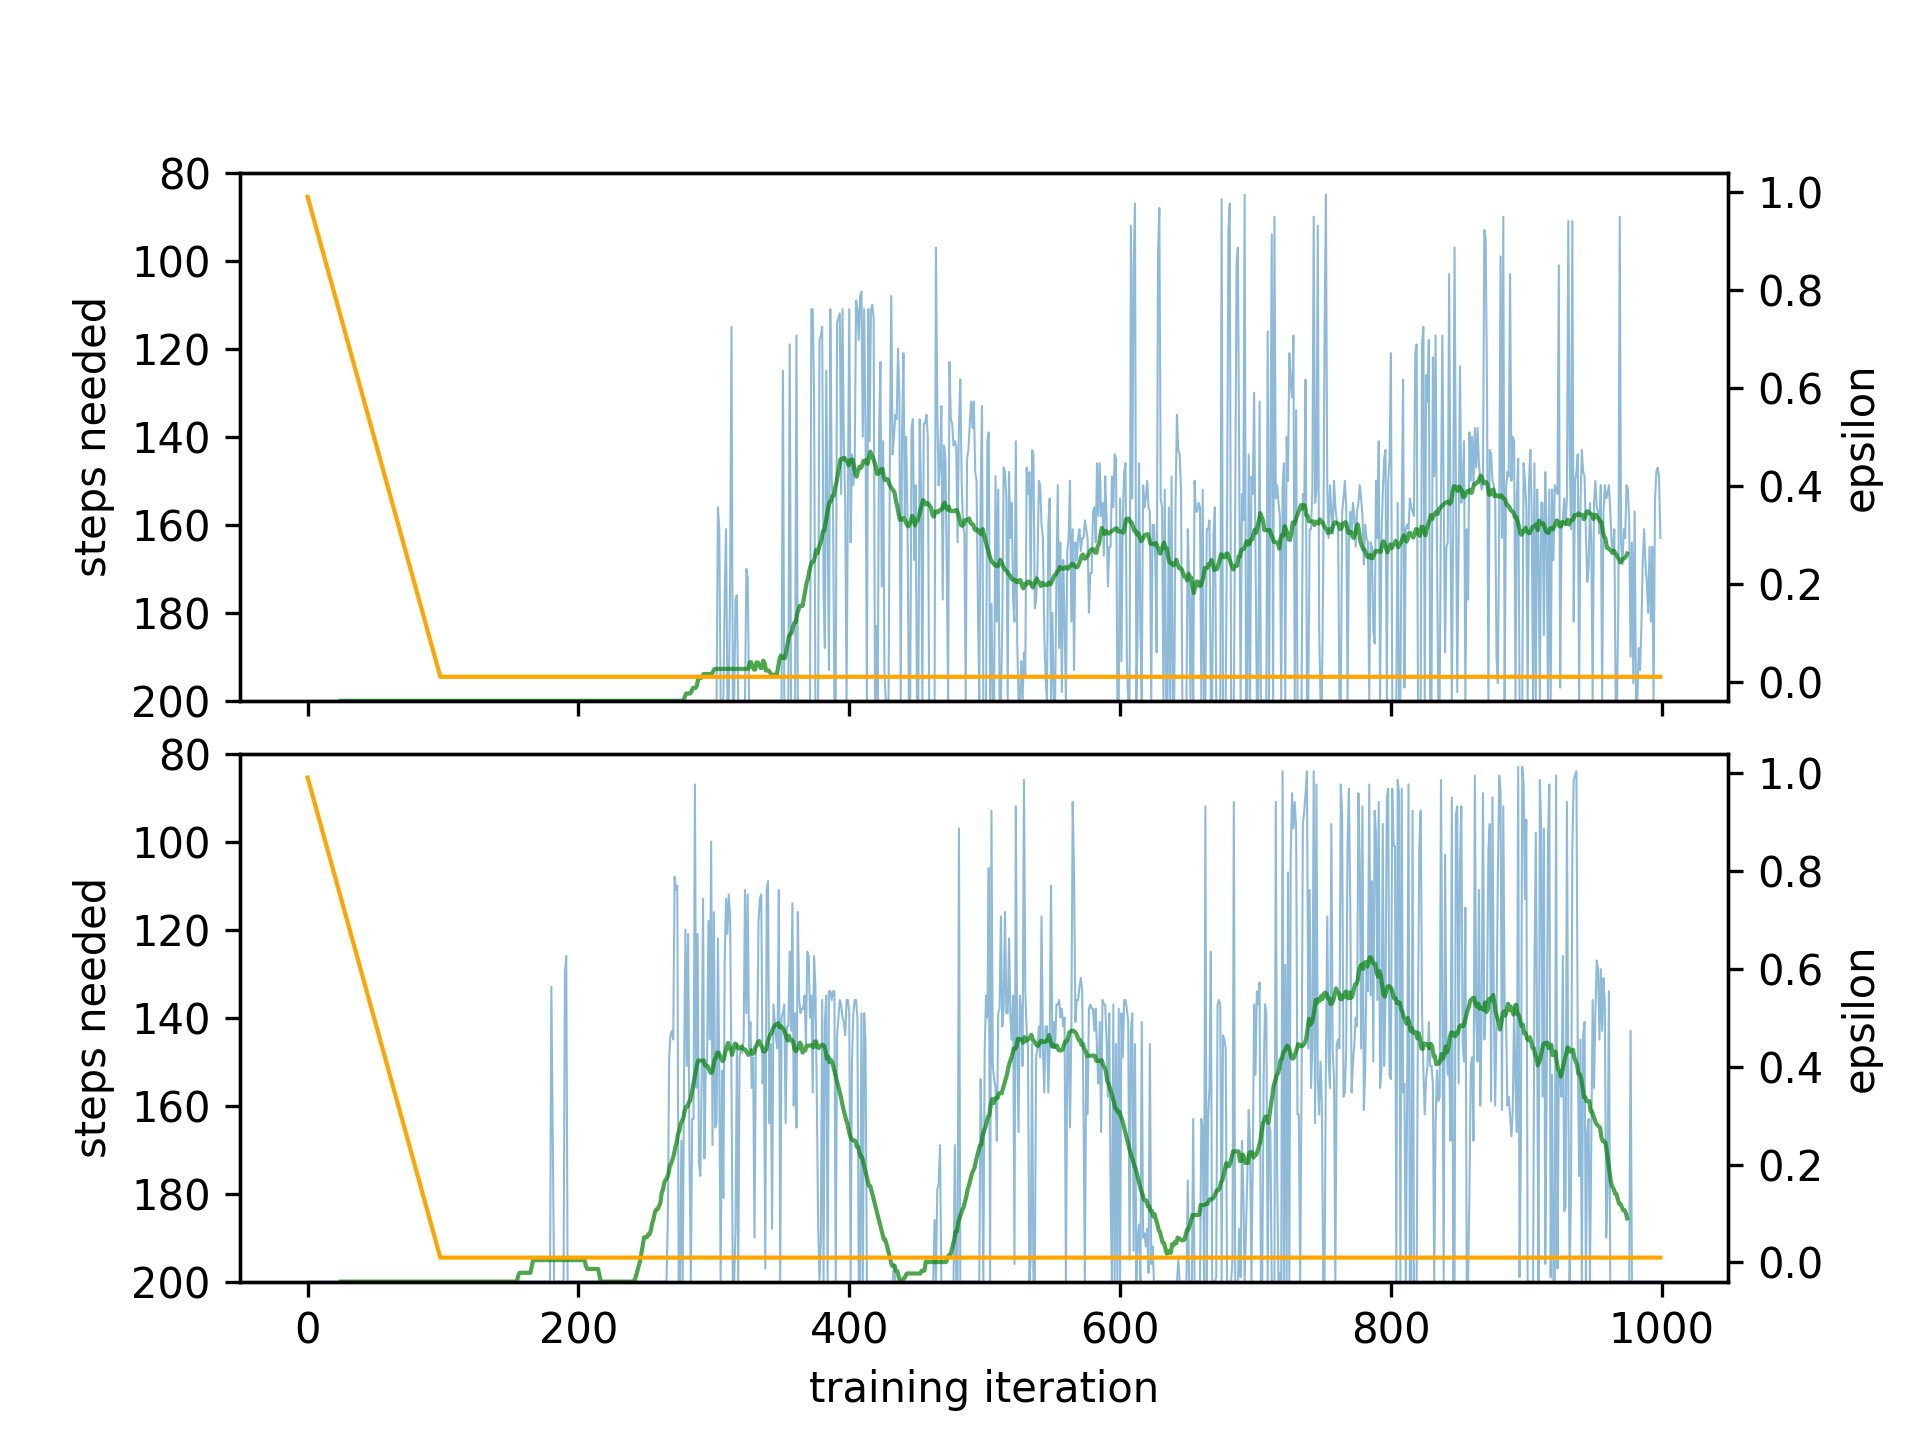
\includegraphics{mcar_40000_a}
    \caption{Two separate runs of training the mountain car agent with a replay buffer which remembers the last $40000$ time steps. On the y-axis the number of steps needed to finish, 200 means the algorithm failed to reach the goal in time. On the x-axis the iteration number. The orange line is epsilon, the blue line follows the scores of the training iteration and the green line is the moving average of the score. Note the agent solves the problem in most training iterations}
    \label{fig:mcar_40k_a}
\end{figure}

\begin{figure}
    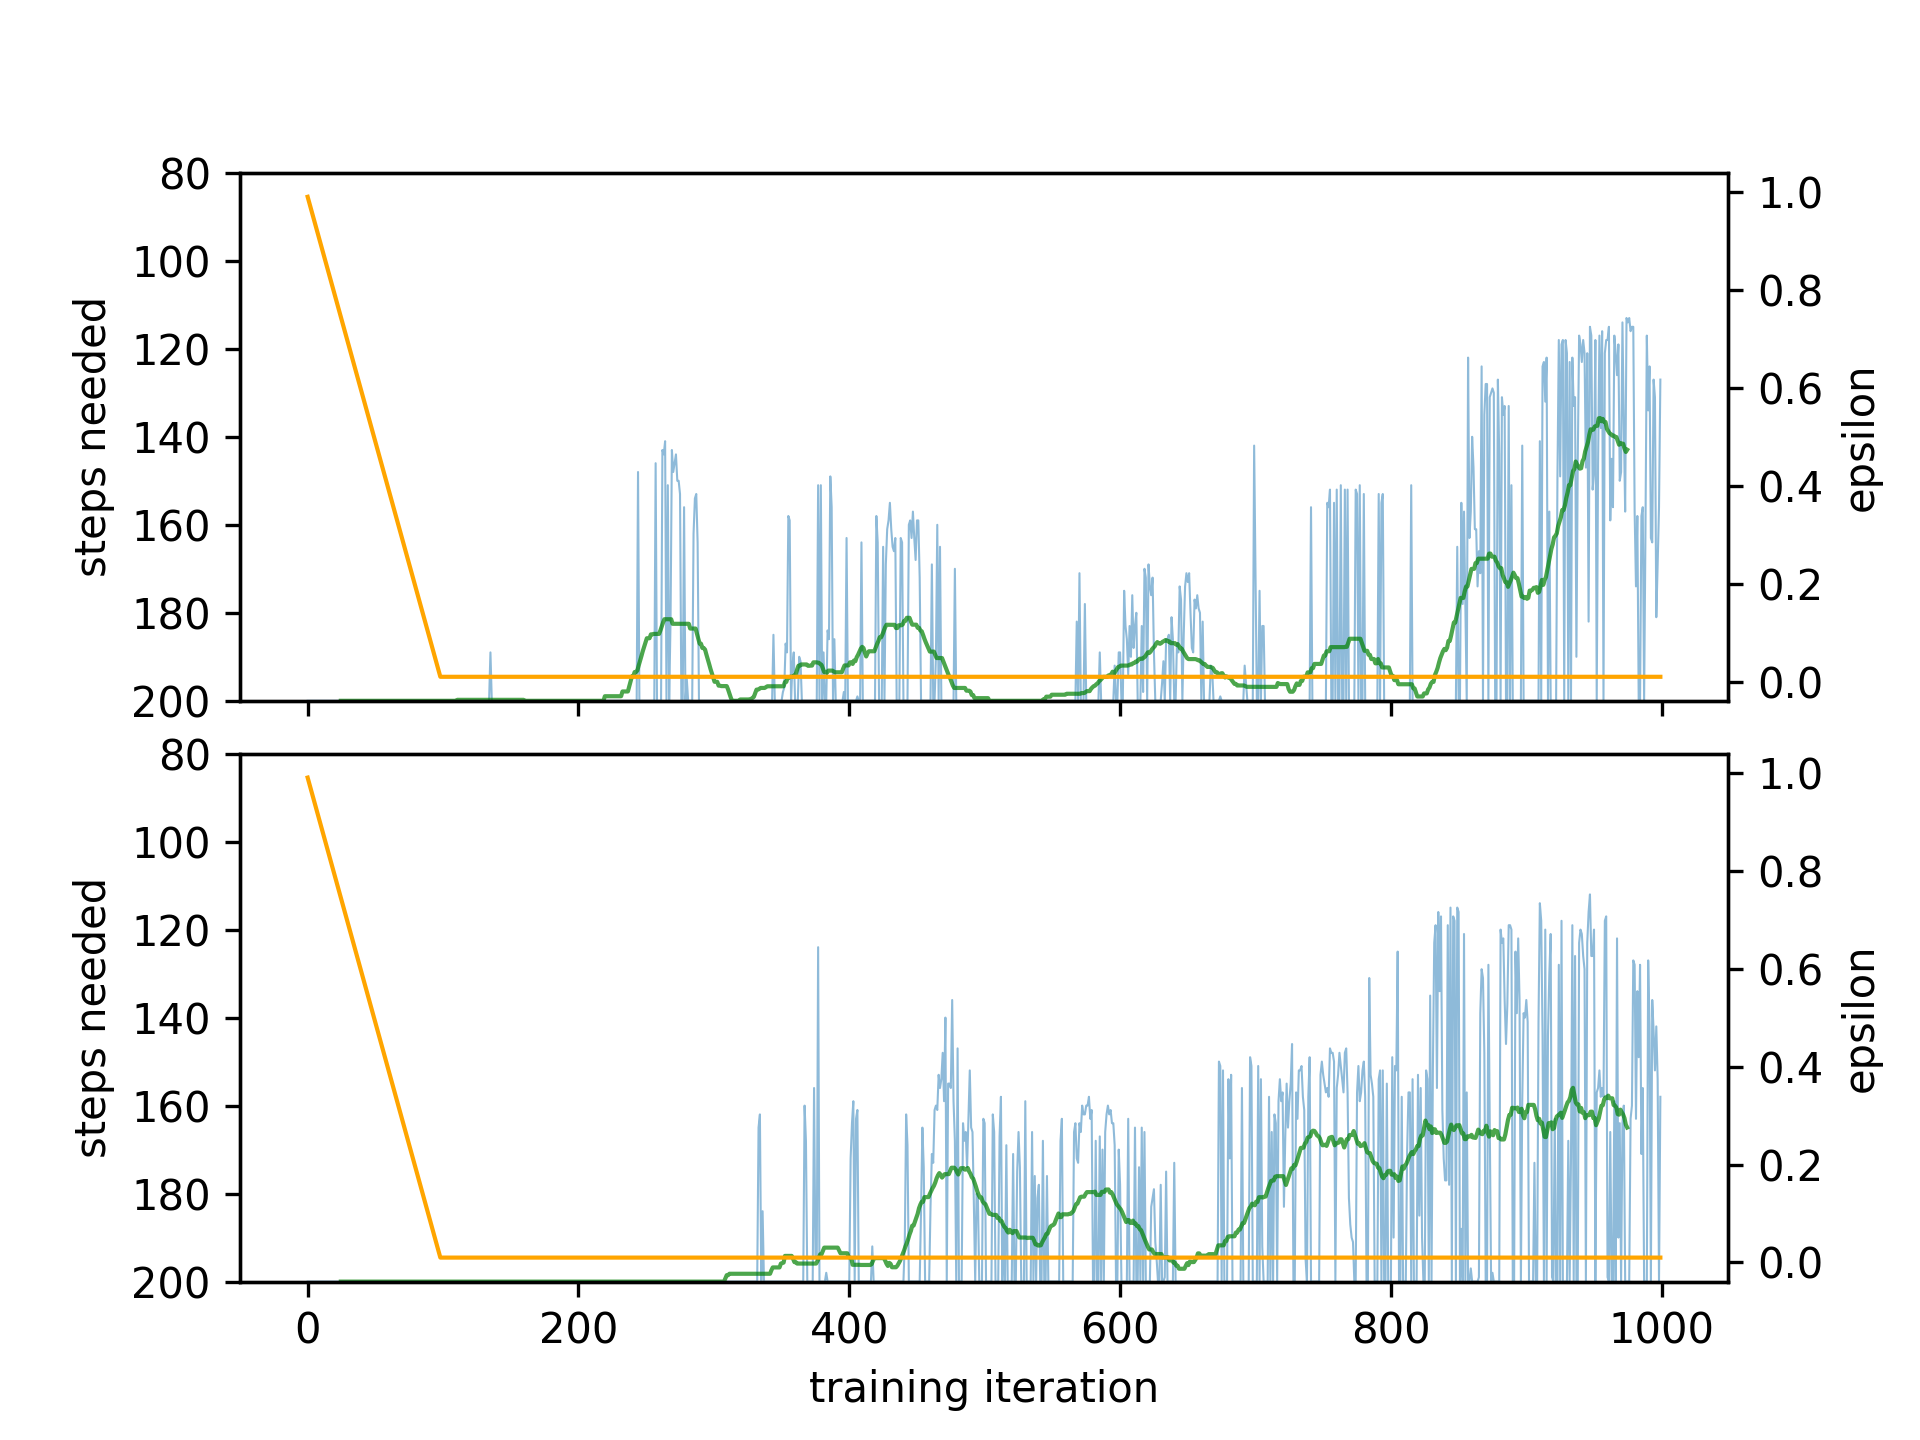
\includegraphics{mcar_40000_b}
    \caption{Two separate runs of training the mountain car agent with a replay buffer which remembers the last $40000$ time steps. On the y-axis the number of steps needed to finish, 200 means the algorithm failed to reach the goal in time. On the x-axis the iteration number. The orange line is epsilon, the blue line follows the scores of the training iteration and the green line is the moving average of the score. Here the agent solves the problem often but it is very inefficient in doing so}
    \label{fig:mcar_40k_b}
\end{figure}

We see that with the larger replay buffer the agent performs okay in more scenarios it also was able to solve the task every time I trained the agent from scratch. The overall performance however is worse compared to the other successful training runs as seen best in \autoref{fig:mcar_40k_b}.

Now I compare two mountain car agent with both a replay buffer of size $40 000$\footnote{we pick this size over the default $20 000$ as it performs more reliably}. To do this I do two more runs at $40 000$ however the agent trains the same neural network network as it uses for predictions\footnote{the copying of weights is also disabled as we are no longer using the separate train network and copying its random weights would make training the network useless}. I expect this to cause the agent to destabilize more.

After running the training 4 times the agent was able to reach the goal in only one run, in the other 3 the number of steps needed stayed at $200$ for all $1000$ training iterations. The successful run is presented in \autoref{fig:no_iwu}.

\begin{figure}
    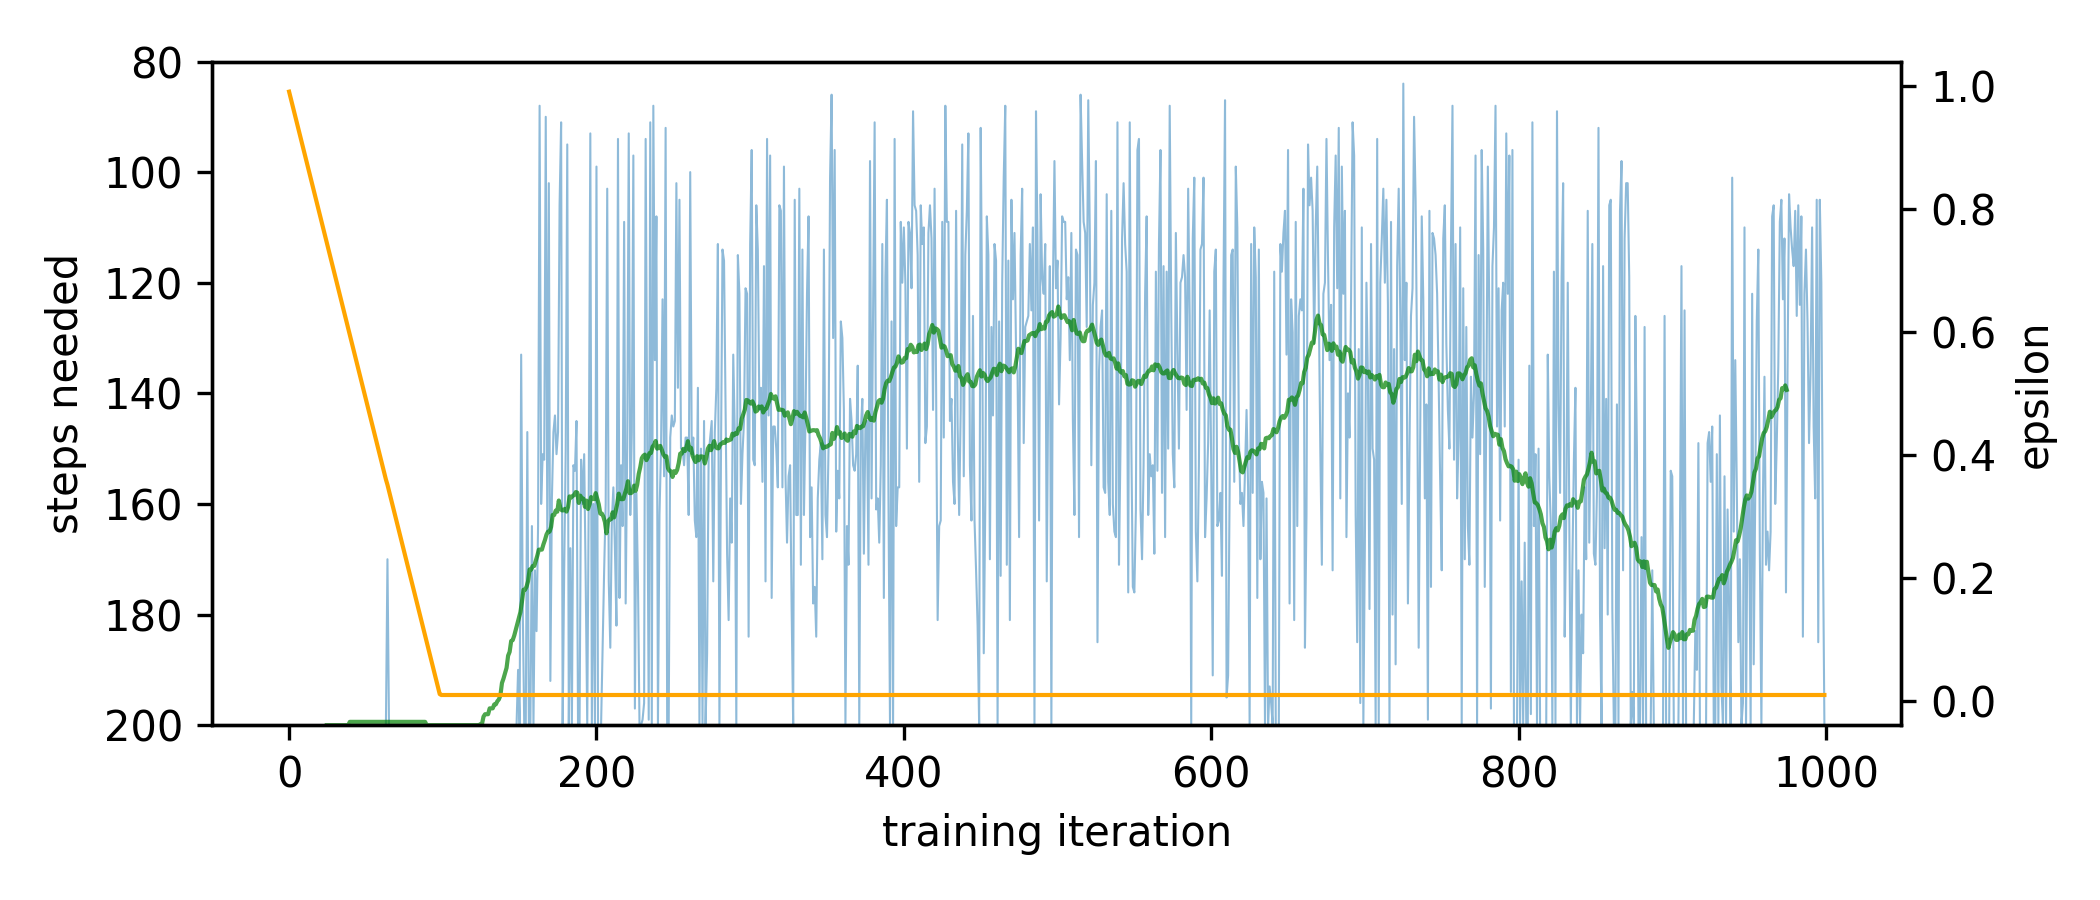
\includegraphics{mcar_40000_no_iwu}
    \caption{The training of the agent with a replay buffer (size: $40000$ time steps) but without infrequent weights updates. On the y-axis the number of steps needed to finish, 200 means the algorithm failed to reach the goal in time. On the x-axis the iteration number. The orange line is epsilon, the blue line follows the scores of the training iteration and the green line is the moving average of the score. The agent solves the problem after less then 200 training iterations}
    \label{fig:no_iwu}
\end{figure}

We see the agent learned really quickly, which is to be expected since the actions are immediately based on newly learned behavior. However this plot also seems to show slightly more stable performance, as it performs really well for most iterations this is counter intuitive. A possible explanation could be the network adapting quickly or this training run being a particularly easy one due to random chance.